\documentclass[ignorenonframetext,xcolor=x11names]{beamer}

\input{../common.preamble.beamer.tex}

\title{Business 4720 - Class 14}

\subtitle{Time Series}

\begin{document}

\begin{frame}{}
  \titlepage
  \footnotesize
  \input{../license.tex}
\end{frame}

\section{Introduction}

\begin{frame}{This Class}

\begin{block}{What You Will Learn:}
\begin{itemize}
  \item Time Series Models
  \begin{itemize}
     \item Time series basics
     \item Smoothing methods
     \item ARIMA models
     \item Seasonal models
     \item GARCH Models
  \end{itemize}
\end{itemize}
\end{block}
\end{frame}


\begin{frame}{Based On}
\small
\begin{block}{}
Robert H. Shumway and David S. Stoffer (2017) \emph{Time Series Analysis and Its Applications}, 4th Edition. Springer. \url{https://www.stat.pitt.edu/stoffer/tsa4/} \\

\vspace{\baselineskip}
Rob J. Hyndman and George Athanasopoulos (2018) \emph{Forecasting: Principles and Practice}, 2nd edition. OTexts. \url{https://otexts.com/fpp2/} 
\end{block}

\begin{block}{Useful Tutorials}
\begin{itemize}
\item \url{https://github.com/nickpoison/tsa4}
\item \url{https://a-little-book-of-r-for-time-series.readthedocs.io/en/latest/src/timeseries.html}
\item \url{https://rc2e.com/timeseriesanalysis}
\item \url{https://atsa-es.github.io/atsa-labs/chap-tslab.html}
\end{itemize}
\end{block}

\end{frame}

\begin{frame}{Time Series Application Examples}
\begin{itemize}
  \item Finance: Stock market predictions
  \item Economics: Unemployment rates
  \item Social science: School enrollment
  \item Natural sciences: Global temperature trends
  \item Ecology: Fish population forecasting
  \item Epidemiology: COVID incidence rates
\end{itemize}
\centering

\includegraphics[width=\textwidth]{figure1.pdf}
\end{frame}


\begin{frame}{Characteristics of Time Series}
\begin{block}{Time-Domain Approach}
\begin{itemize}
  \item Focuses on lagged relationships
  \item \emph{Example}: How does yesterday's stock performance affect today's stock performance?
\end{itemize}
\end{block}

\begin{block}{Frequency-Domain Approach}
\begin{itemize}
  \item Focuses on cycles
  \item \emph{Example}: What is the economic cycle through periods of expansion and recession?
\end{itemize}
\end{block}
\end{frame}

\begin{frame}{Time Series Statistical Models}
\begin{itemize}
   \item Moving Averages
   \item Autoregressive Model
   \item Random walk with drift
   \item Signal in noise
\end{itemize}
\end{frame}

\begin{frame}[fragile]{Moving Averages}
Example:
\begin{align*}v_t = \frac{1}{3} ( w_{t-1} + w_t + w_{t+1})\end{align*}
\begin{Rcode}
# Load ASTSA library
library(astsa)

# Random numbers
w = rnorm(500,0,1)

# Moving average
v = filter(w, sides=2, filter=rep(1/3,3))

# Plot timeseries
par(mfrow=c(2,1))
tsplot(w, ylim=c(-3,3), main="white noise", col=3)
tsplot(v, ylim=c(-3,3), main="moving average", col=4)
\end{Rcode}
\end{frame}

\begin{frame}{Moving Averages \small [cont'd]}
\centering

\includegraphics[width=.75\textwidth]{figure2.pdf}
\end{frame}

\begin{frame}[fragile]{Autoregressions}
Example:
\begin{align*}x_t = x_{t-1} - 0.9 x_{t-2} + w_t\end{align*}
\begin{Rcode}
# Random numbers (errors)
w = rnorm(550,0,1)

# Autoregressive time series
x = filter(w, filter=c(1,-.9), method="recursive")

# Remove first 50 values for startup
x = x[-(1:50)]

# Plot time series
tsplot(x, main="autoregression", col=4)
\end{Rcode}
\end{frame}

\begin{frame}{Autoregressions \small [cont'd]}
\centering

\includegraphics[width=\textwidth]{figure3.pdf}
\end{frame}

\begin{frame}[fragile]{Random Walk with Drift}
\begin{columns}
\begin{column}{.4\textwidth}
Example:
\begin{align*}x_t &= \delta + x_{t-1} + w_t \\
&= \delta t + \sum_{j=1}^t w_j\end{align*}
\end{column}
\begin{column}{.7\textwidth}
\begin{Rcode}
# White noise
w = rnorm(200)
# Random walk
x = cumsum(w)

# Drift
drift = .2
# White noise with drift
w.drift = w + drift;
# Random walk with drift
x.drift = cumsum(w.drift)

# Plot
tsplot(x.drift, main="random walk", col=3, 
       ylab='', ylim=c(-10,55))
abline(a=0, b=drift, lty=2, col=3)
lines(x, col=4)
abline(a=0, b=0, lty=2, col=4)
\end{Rcode}
\end{column}
\end{columns}
\end{frame}

\begin{frame}{Random Walk with Drift \small [cont'd]}
\includegraphics[width=\textwidth]{figure4.pdf}
\end{frame}

\begin{frame}[fragile]{Signal in Noise}
Example:
\begin{align*}
x_t &= A \cos (2 \pi \omega t + \phi) \\
A &= 2 &\qquad \text{amplitude} \\
\omega &= 1/50 &\qquad \text{frequency} \\
\phi &= .6 \pi &\qquad \text{phase shift}
\end{align*}

\vspace{-1.5\baselineskip}
\begin{Rcode}
# Create signal
cs = 2*cos(2*pi*1:500/50 + .6*pi)

# Create noise
w = rnorm(500,0,1)

# Plot signal with different amount of noise
par(mfrow=c(3,1), mar=c(3,2,2,1), cex.main=1.5)
tsplot(cs, main='Signal', col=2)
tsplot(cs+w, main='Signal and N(0,1) noise', col=3)
tsplot(cs+5*w, main='Signal and N(0,25) noise', col=4)
\end{Rcode}
\end{frame}

\begin{frame}{Signal in Noise \small [cont'd]}
\centering
\includegraphics[width=.75\textwidth]{figure5.pdf}
\end{frame}

\begin{frame}[fragile]{Basic Time Series Operations in R}
Building a time series:
\begin{Rcode}
# Creating a time series object with monthly data
ts_data <- ts(1:24, frequency = 12, start = c(2020, 1))
\end{Rcode}
Dealing with missing values:
\begin{Rcode}
library(zoo)

# Introduce NA values
ts_data[c(5, 10, 15)] <- NA

# Remove leading/trailing NA values
trimmed_ts <- na.trim(ts_data)

# Last Observation Carried Forward
locf_ts <- na.locf(ts_data)

# Interpolate NA values
approx_ts <- na.approx(ts_data)
\end{Rcode}
\end{frame}

\begin{frame}[fragile]{Basic Time Series Operations in R}
First and last observations:
\begin{Rcode}
head(ts_data)
tail(ts_data)
\end{Rcode}
Merging time series:
\begin{Rcode}
# Creating another time series
ts_data2 <- ts(c(1:24), frequency = 12, start = c(2020, 7))

# Find intersection of two time series
intersect_ts <- ts.intersect(ts_data, ts_data2)

# Find union of two time series
union_ts <- ts.union(ts_data, ts_data2)
\end{Rcode}
\end{frame}

\begin{frame}[fragile]{Basic Time Series Operations in R}
Lagging a series (shifting forward or backward in time):
\begin{Rcode}
# Positive k shifts backwards
lag(ts_data, 6)

# Negative k shifts forwards
lag(ts_data, -3)
\end{Rcode}
\end{frame}

\begin{frame}{Smoothing a Time Series}
\begin{itemize}
   \item Moving average
   \item Kernel smoothing
   \item KNN regression / Lowess
   \item Smoothing splines
\end{itemize}
\end{frame}

\begin{frame}[fragile]{Moving Average}
\begin{align*}m_t = \sum_{j=-k}^k a_j x_{t-j} \quad \text{where} \quad
\sum_{j=-k}^k a_j = 1
\end{align*}
\begin{Rcode}
f = c(.5, rep(1, 11), .5)/12
filter(soi, sides=2, filter=f)
\end{Rcode}
\begin{center}
\includegraphics[width=.75\textwidth]{figure14.pdf}
\end{center}
\end{frame}

\begin{frame}[fragile]{Kernel Smoothing}
\begin{align*}a_i(t) = K\left(\frac{t-i}{b}\right) / \sum_{j=1}^n K \left(\frac{t-j}{b}\right) \; \text{and} \; K(z) = \frac{1}{\sqrt{2\pi}} \exp(-z^2/2) \end{align*}
\begin{Rcode}
ksmooth(time(soi), soi, 'normal', bandwidth=1)
\end{Rcode}
\begin{center}
\includegraphics[width=.75\textwidth]{figure15.pdf}
\end{center}
\end{frame}

\begin{frame}[fragile]{Locally Weighted Regression}
\begin{itemize}
   \item Identify proportion $f$ of closest points
   \item Use weighted least squares regression to predict values
\end{itemize}
\begin{Rcode}
lowess(soi, f=0.1)
\end{Rcode}
\begin{center}
\includegraphics[width=.75\textwidth]{figure16.pdf}
\end{center}
\end{frame}

\begin{frame}[fragile]{Smoothing Splines}
\begin{itemize}
  \item Penalized polynomial regression
  \item Fit $m_t = \beta_0 + \beta_1 t + \beta_2 t^2$
  \item Minimize loss function:
\begin{align*}
\sum_{t=1}^n (x_t - m_t)^2 + \lambda \int \left( \dv[2]{m}{t} \right)^2 \, dt
\end{align*}
\end{itemize}
\begin{Rcode}
smooth.spline(time(soi), soi, spar=0.5)
\end{Rcode}
\vspace{-1.5\baselineskip}
\begin{center}
\includegraphics[width=.75\textwidth]{figure17.pdf}
\end{center}
\end{frame}


\begin{frame}{Hands-On Exercises}
\begin{enumerate}
   \item Generate 100 observations from the autoregression model $x_t = -.9x_{t-2} + w_t$ with $\sigma^2_w = 1$
  \begin{enumerate}
     \item Smooth the time series using a moving average filter $v_t = (x_t + x_{t-1} + x_{t-2} + x_{t-3})/4$
     \item Plot $x_t$ as a line and superimpose $v_t$
     \item Comment on the behaviour of $x_t$ and how applying the moving average filter changes that behavior
  \end{enumerate}
  \item Repeat the smoothing but with $x_t = \cos(2 \pi t / 4)$
  \item Repeat the smoothing but with added $N(0,1)$ noise, that is smooth $x_t = \cos(2\pi t /4) + w_t$
  \item Compare and contrast the three exercises: How does the moving average change each series
\end{enumerate}
\hrule
\footnotesize
\begin{itemize}
  \item Use \texttt{x = filter(w, filter=c(a, b), method="recursive")}
  \item Use \texttt{v = filter(x, rep(1/4, 4), sides=1)} as above.
  \item Use \texttt{c = cos(2*pi*1:500/4)} as above.
  \item Use \texttt{lines(...,lty=2)} to add lines to a plot
\end{itemize}
\end{frame}


\begin{frame}[fragile]{Time Series Regression Example}
Epidemiology Example:
\begin{itemize}
  \item Cardiovascular mortality \texttt{cmort}
  \item Temperate \texttt{tempr}
  \item Particulate pollution \texttt{part}
\end{itemize}

\begin{Rcode}
# IMPORTANT: Use ts.plot, NOT tsplot:
ts.plot(cmort, tempr, part, col=2:4)
\end{Rcode} 

\vspace{-2\baselineskip}
\includegraphics[width=1.05\textwidth]{figure11.pdf}
\end{frame}

\begin{frame}[fragile]{Time Series Regression Example \small [cont'd]}
Fit different linear regression models (at the same time points):
\begin{Rcode}
# Center Temperature
temp = tempr - mean(tempr)

# Square Temperature
temp.2 = temp^2

# Fit different linear models and provide summaries
summary(lm(cmort ~ time(cmort)))
summary(lm(cmort ~ time(cmort) + temp))
summary(lm(cmort ~ time(cmort) + temp + temp.2))
summary(lm(cmort ~ time(cmort) + temp + temp.2 + part))
\end{Rcode}
\end{frame}

\begin{frame}[fragile]{Time Series Regression Example}{With Lagged Variables}

\begin{Rcode}
# Lag the temperature
temp.l.2 = lag(temp, 2)
temp.l.4 = lag(temp, 4)

# Intersect all time series to
# omit leading/trailing NA
temp.df <- ts.intersect(cmort, time(cmort), part, 
                        temp, temp.2, temp.l.2, 
                        temp.l.4,
                        dframe=TRUE)
# Fit the linear model including lagged temperature
summary(lm(cmort ~ time.cmort. + temp + temp.2 + 
                   temp.l.2 + temp.l.4 + part, 
           data=temp.df))
\end{Rcode}
\end{frame}


\begin{frame}{Strict Stationarity}
A \textbf{strictly stationary} time series is one for which the probabilistic behaviour of every collection of values
\begin{align*}&\{x_{t_1}, x_{t_2}, \ldots, x_{t_k} \} \\
\intertext{is identical to that of the shifted set}
&\{x_{t_1+h}, x_{t_2+h}, \ldots, x_{t_k + h} \}. \\
\intertext{That is,}
&\Pr \{ x_{t_1} \leq c_1, \ldots, x_{t_k} \leq c_k \} = \Pr \{ x_{t_1+h}\leq c_1, \ldots , x_{t_k+h} \leq c_k \}
\end{align*}
\end{frame}

\begin{frame}{Measures of Dependence}
\begin{block}{Autocovariance}
\begin{itemize}
   \item Covariance between two points $t, t+h$ on time series $x$ 
\begin{align*}
\gamma(h) = cov(x_t, x_{t+h}) = E [ (x_t - \mu)(x_{t+h} - \mu)] 
\end{align*}
\vspace{-\baselineskip}
   \item Large autocovariance $\rightarrow$ smooth time series
   \item Small autocovariance $\rightarrow$ choppy time series
\end{itemize}
\end{block}
\begin{block}{Sample Autocovariance for Lag \emph{h}}
\begin{align*}
\hat{\gamma}(h)  = \frac{1}{(q-p)} \sum_{t=p}^{q-h} (x_t - \bar{x})(x_{t+h} - \bar{x})
\end{align*}
\end{block}
\end{frame}

\begin{frame}{Measures of Dependence \small [cont'd]}
\begin{block}{Autocorrelation Function (ACF)}
\begin{align*}
\rho_x(h) = \frac{\gamma (t+h,t)}{\sqrt{\gamma (t+h,t+h) \gamma(t, t)}} = \frac{\gamma(h)}{\gamma(0)}  \quad \text{\small (weak stationarity)}
\end{align*}
\end{block}
\begin{block}{Sample Autocorrelation for Lag \emph{h}}
\begin{align*}
\hat\rho_x(h) = \frac{\hat\gamma(h)}{\sqrt{\hat\gamma(h) \hat\gamma(0)}} = \frac{\hat\gamma(h)}{\hat\gamma(0)} \quad \text{\small (weak stationarity)}
\end{align*}
\end{block}
\end{frame}


\begin{frame}{Weak Stationarity}
A \textbf{weakly stationary} time series is a process such that
\begin{enumerate}
\item the mean is constant and does not depend on time: $\mu_t = \mu$
\item the autocovariance $\gamma$ depends on $s$ and $t$ only through their difference $h=|s-t|$.
\end{enumerate}
Let $s = t + h$, then:
\begin{align*}
\gamma(s, t) = \gamma(t+h, t) &= cov(x_{t+h}, x_t) = cov(x_h, x_0) = \gamma(h) \\
\intertext{and}
\rho(h) &= \gamma(h) / \gamma(0)
%\intertext{and the CCF of two jointly stationary time series is}
%\rho_{xy}(h) &= \frac{\gamma_{xy}(h)}{\sqrt{\gamma_x(0)\gamma_y(0)}}
\end{align*}
\end{frame}

\begin{frame}{Measures of Dependence \small [cont'd]}
The large-sample distribution of $\hat{\rho}_{x}(h)$ is normal with mean $0$ and standard deviation
\begin{align*}
\sigma_{\hat{\rho}_{x}} = 1/ \sqrt{n} 
\end{align*}
\emph{if the processes is independent white noise}. \\

Hence, the approximate 95\% confidence interval on the ACF is
\begin{align*}
-\frac{1}{n} \pm \frac{2}{\sqrt{n}}
\end{align*}
\end{frame}

%\begin{frame}[fragile]{Standard Deviations of ACF and CCF}
%\small
%\begin{enumerate}
%\item The large sample distribution of the auto-covariance function $\hat{\rho}_{x}(h)$ is normal with mean zero and standard deviation
%\begin{align*}
%\sigma_{\hat{\rho}_{x}} = 1/ \sqrt{n} 
%\end{align*}
%if the processes is independent white noise.

%\item The large sample distribution of the cross-covariance function $\hat{\rho}_{xy}(h)$ is normal with mean zero and standard deviation
%\begin{align*}
%\sigma_{\hat{\rho}_{xy}} = 1/ \sqrt{n} 
%\end{align*}
%if at least one of the processes is independent white noise.
%\end{enumerate}
%This allows \emph{significance testing} of ACF and CCF through $\pm 2/\sqrt{N}$ intervals in which $95\%$ of samples should be found.
%\end{frame}


\begin{frame}[fragile]{Autocorrelation Function (ACF) Example 1}
Gaussian white noise example:
\begin{Rcode}
library(astsa)
t <- ts(rnorm(500))

# The hard way:
cor(ts.intersect(t, lag(t,1), dframe=T))
cor(ts.intersect(t, lag(t,2), dframe=T))
# etc.

# The easy way:
# Without plot
acf <- acf1(t, plot=FALSE)
# With plot
acf1(t, col=7, lwd=3)
\end{Rcode}
\end{frame}

\begin{frame}{Autocorrelation Function (ACF) Example 1 \small [cont'd]}
\begin{center}
\includegraphics[width=\textwidth]{figure7a.pdf}
\end{center}
\end{frame}

\begin{frame}[fragile]{Autocorrelation Function (ACF) Example 2}
Example using the \texttt{soi} data set (sea level air pressure index) from the \texttt{astsa} library:
\begin{Rcode}
library(astsa)

# Compute and plot the ACF for different lags
acf1(soi, co=3, lwd=2)

# Scatterplot of original versus or lags up to 6, with ACF
lag1.plot(soi, max.lag = 6, col=4, lwl=3)
\end{Rcode}
\end{frame}

\begin{frame}{Autocorrelation Function (ACF) Example 2 \small [cont'd]}
\centering
\includegraphics[height=3.25in]{figure8a.pdf}
\end{frame}

%\begin{frame}{Measures of Dependence}
%\begin{block}{Cross-covariance}
%\begin{align*}
%\gamma_{xy}(s, t) = cov(x_s, y_t) = E [ (x_s - \mu_{xs})(y_t - \mu_{yt})]
%\end{align*}
%\end{block}
%\begin{block}{Cross-correlation (CCF)}
%\begin{align*}
%\rho_{xy}(s, t) = \frac{\gamma_{xy} (s,t)}{\sqrt{\gamma_x (s,s) \gamma_y(t, t)}}
%\end{align*}
%\end{block}
%\end{frame}

%\begin{frame}[fragile]{Cross-Correlation Function}
%Gaussian white noise example:
%\begin{Rcode}
%x = rnorm(100)
%y = lag(x, -5) + rnorm(100)
%ccf2(y, x, ylab='CCF', gg=T, col=4)
%\end{Rcode}
%\begin{center}
%\includegraphics[width=.85\textwidth]{figure6.pdf}
%\end{center}
%\end{frame}

%\begin{frame}[fragile]{Cross-Correlation Function}
%Example using the \texttt{soi} air pressure index and the \texttt{rec} data (''recruitment'', i.e. new fish index) from the \texttt{astsa} library:
%\begin{Rcode}
%par(mfrow=c(3,1))
%acf1(soi, 48, main="SOI", gg=T, col=2)
%acf1(rec, 48, main="New Fish", gg=T, col=3)
%ccf2(soi, rec, 48, main="SOI vs New Fish", 
     %ylab="CCF", gg=T, col=4)
%\end{Rcode}
%\end{frame}

%\begin{frame}{Cross-Correlation Function}
%\centering

%\includegraphics[width=.7\textwidth]{figure9.pdf}
%\end{frame}

%\begin{frame}[fragile]{Pre-Whitening}
%\emph{To use $95\%$ intervals for significance testing of CCF, one series must be white noise.} \\

%\textbf{Example:} Generate two independent cyclical time series (signal plus error):
%\begin{Rcode}
%num=120; t=1:num
%X = ts(2*cos(2*pi*t/12) + rnorm(num), freq=12)
%Y = ts(2*cos(2*pi*(t+5)/12) + rnorm(num), freq=12)
%\end{Rcode}
%Residualize $Y$ on $X$ to remove the $X$ signal from $Y$:
%\begin{Rcode}
%Yw = resid( lm(Y~ cos(2*pi*t/12) + sin(2*pi*t/12), 
                                     %na.action=NULL))
%\end{Rcode}
%\end{frame}

%\begin{frame}[fragile]{Pre-Whitening}
%\begin{Rcode}
%par(mfrow=c(3,2), mgp=c(1.6,.6,0), mar=c(3,3,1,1) )
%tsplot(X, gg=T, col=3)
%tsplot(Y, gg=T, col=4)
%acf1(X,48, ylab='ACF(X)', gg=T, col=3)
%acf1(Y,48, ylab='ACF(Y)', gg=T, col=4)
%ccf2(X,Y,24, ylab='CCF(X,Y)', gg=T)
%ccf2(X,Yw,24, ylab='CCF(X,Yw)', ylim=c(-.6,.6), gg=T)
%\end{Rcode}
%\end{frame}

%\begin{frame}{Pre-Whitening}
%\centering

%\includegraphics[height=3in]{figure10.pdf}
%\end{frame}

\begin{frame}{Dealing with Non-Stationarity}
\begin{block}{Log Transformation}
  \begin{align*}y_t = \log x_t\end{align*}
\end{block}
\begin{block}{Box-Cox power transformation}
  \begin{align*}y_t = \begin{cases}(x_t^\lambda-1)/\lambda &\quad \lambda\neq0 \\
  \log x_t &\quad \lambda=0
  \end{cases}
  \end{align*}
\end{block}
\end{frame}


\begin{frame}[fragile]{Dealing with Non-Stationarity}
Assume that $x_t = \mu_t + y_t$ where $\mu_t$ is the trend and $y_t$ a stationary process.
\begin{block}{Detrending}
\begin{itemize}
  \item Estimate trend, e.g. with an LM such as $\mu_t = \beta_0 + \beta_1 t$
  \item Work with residuals, e.g. $\hat y_t = x_t - \hat \mu_t = x_t - \hat\beta_0 - \hat\beta_1 t$
\end{itemize}
\end{block}
\begin{Rcode}
# Simulate a time series with a linear trend
t <- ts(1:100 + rnorm(100) * 10)

# Fit a linear model to the time series
trend_model <- lm(t ~ time(t))
# Calculate detrended series
detrended <- residuals(trend_model)

# Plot original and detrended
par(mfrow=c(2,1))
tsplot(t, type="l", main="original", col=3)
tsplot(detrended, type="l", main="detrend", col=2)
\end{Rcode}
\end{frame}

\begin{frame}{Detrending Example}
\centering
\includegraphics[width=.9\textwidth]{figure39a.pdf}
\end{frame}


%\begin{frame}{Dealing with Non-Stationarity}
%Assume that $x_t = \mu_t + y_t$ where $\mu_t$ is the trend and $y_t$ a stationary process.
%\begin{block}{Detrending}
%\begin{itemize}
  %\item Estimate trend, e.g. with an LM such as $\mu_t = \beta_0 + \beta_1 t$
  %\item Work with residuals, e.g. $\hat y_t = x_t - \hat \mu_t = x_t - \hat\beta_0 - \hat\beta_1 t$
%\end{itemize}
%\end{block}

%\begin{block}{Differencing}
%\begin{itemize}
  %\item Model trend stochastically as random walk with drift: $\mu_t = \delta + \mu_{t-1} + w_t$ where $w_t$ is white noise
  %\item Differencing then yields $x_t - x_{t-1} = (\mu_t + y_t) - (\mu_{t-1} + y_{t-1}) = \delta + w_t + y_t - y_{t-1}$ which is stationary
%\end{itemize}
%\end{block}
%\end{frame}

\begin{frame}{Dealing with Non-Stationarity}
Assume that $x_t = \mu_t + y_t$ where $\mu_t$ is the trend and $y_t$ a stationary process.
\begin{block}{Differencing}
\begin{itemize}
  \item Model the trend stochastically as a random walk with drift: $\mu_t = \delta + \mu_{t-1} + w_t$ where $w_t$ is white noise
  \item Differencing then yields 
  \begin{align*}x_t - x_{t-1} &= (\mu_t + y_t) - (\mu_{t-1} + y_{t-1})  \\
  &= \mu_t - \mu_{t-1} + y_t - y_{t-1} \\
  &= \delta + w_t + y_t - y_{t-1}
  \end{align*}
  which is stationary
\end{itemize}
\end{block}
\begin{itemize}
  \item First difference eliminates linear trend
  \item Second difference eliminates quadratic trend
  \item \ldots
\end{itemize}
\end{frame}

\begin{frame}[fragile]{Differencing in R}
\begin{Rcode}
set.seed(42)
# Simulating a time series with trend
t <- ts(cumsum(rnorm(100))) 

# Plot original, first, and second difference
par(mfrow=c(3,1))
tsplot(t, type="l", 
    main="original", col=3)

tsplot(diff(t, differences = 1), type="l", 
    main="first difference", col=4)

tsplot(diff(t, differences = 2), type="l", 
    main="second difference", col=5)
\end{Rcode}
\end{frame}

\begin{frame}{Differencing in R}
\begin{center}
\includegraphics[height=3in]{figure40a.pdf}
\end{center}
\end{frame}

\begin{frame}[fragile]{Detrending and Differencing in R -- ACF}
Compare the ACF of the original, detrended, and differenced series:
\begin{Rcode}
acf1(chicken, max.lag=48, main="original", col=1)

acf1(resid(fit), max.lag=48, main="detrend", col=2)

acf1(diff(chicken, differences = 1), max.lag=48, 
     main="first diff", col=3)

acf1(diff(chicken, differences = 2), max.lag=48, 
     main="sec diff", col=4)
\end{Rcode}
\end{frame}

\begin{frame}{Detrending and Differencing in R}
\centering
\includegraphics[width=.9\textwidth]{figure41.pdf}
\end{frame}

%\begin{frame}{Detrending and Differencing in R}
%\centering

%\includegraphics[height=3in]{figure13.pdf}
%\end{frame}

\begin{frame}{Hands-On Exercises}
\begin{enumerate}
  \item Extend the mortality, temperature and pollution/particulate model by adding another component to the regression that accounts to the particulate four weeks prior; that is, add $P_{t-4}$ to the regression.
  \item Draw a scatterplot matrix of $M_t$, $T_t$, $P_t$ and $P_{t-4}$, then calculate the pairwise correlations between them. Compare the relationship between $M_t$ and $P_t$ versus $M_t$ and $P_{t-4}$
  \item Detrend the \texttt{soi} time series data by fitting a regression of $S_t$ on time $t$. Is there a significant trend in the surface pressure?
  \item Use two different smoothing techniques to estimate the trend in the global temperature series \texttt{gtemp\_both} in the \texttt{astsa} library.
\end{enumerate}
\end{frame}

\begin{frame}{Hands-On Exercises \small [cont'd]}
Consider the two weekly time series \texttt{oil} and \texttt{gas} in the  \texttt{astsa} library. The oil series is in dollars per barrel, while the gas series in in cents per gallon.
\begin{enumerate}
   \item Plot the data on the same graph. Do you believe the series are stationary?
   \item Apply the transformation $y_t = \nabla \log x_t$ to the data for both series
   \item Plot the transformed series on the same graph, and calculate the ACFs for both series
   \item Plot the CCF of the transformed series and comment.
\end{enumerate}
\end{frame}

\begin{frame}{ARIMA Models}
\begin{itemize}
  \item \textbf{AR}: Autoregressive models
  \item \textbf{MA}: Moving average models
  \item \textbf{ARMA}: Autoregressive moving-average models
  \item \textbf{ARIMA}: Autoregressive integrated moving-average models (for non-stationary models with trend)
\end{itemize}
\end{frame}

\begin{frame}{Differencing \small [cont'd]}
%\begin{block}{Difference Operator}
%\vspace{-\baselineskip}
%\begin{align*}\nabla x_t = x_t - x_{t-1}\end{align*}
%\vspace{-\baselineskip}
%\end{block}
\begin{block}{Backshift / Lag Operator}
\vspace{-\baselineskip}
\begin{align*}\operatorname{B} x_t &= x_{t-1} \\
\operatorname{B}^k x_t &= x_{t-k} % \\
%\nabla x_t &= (1-\operatorname{B})x_t \\
%\nabla^2 x_t &= (1-\operatorname{B})^2 x_t= (1-2 \operatorname{B} + \operatorname{B}^2)x_t = x_t - 2x_{t-1} + x_{t-2} \\
%\nabla^d &= (1-\operatorname{B})^d
 \end{align*}
 \vspace{-\baselineskip}
\end{block}
\end{frame}


\begin{frame}{AR(p) Models}
An \textbf{autoregressive model} of order $p$ is of the form:
\begin{align*}
x_t = \phi_1 x_{t-1} + \phi_2 x_{t-2} + \cdots + \phi_p x_{t-p} + w_t
\end{align*}
where $w_t$ is white noise and $\phi_i$ are model parameters. \\


%\footnotesize
%In contrast to an ''ordinary'' regression model, the $x_i$ are random effects, not fixed, because each $x_i$ has an associated error term $w_t$. \\
%\normalsize

The \textbf{autoregressive operator} $\phi(B)$ is defined using the backshift operator as: 
\begin{align*}
\phi (B) &= 1 - \phi_1 B - \phi_2 B^2 - \cdots - \phi_p B^p \\
         &= \left(1 - \sum_{j=1}^p \phi_j B^j \right)
\end{align*}
so that the AR(p) model becomes:
\begin{align*}
\phi (B) x_t = w_t
\end{align*}
\end{frame}

%\begin{frame}{AR(1) Models}
%The AR(1) model has a stationary solution for $|\phi|<1$, expected value and ACF:
%\begin{align*}
%x_t &= \sum_{j=0}^\infty \phi^j w_{t-j} \\
%E(x_t) &= \sum_{j=0}^\infty \phi^j E(w_{t-j}) = 0 \\
%\rho(h) &= \phi^h = \phi \rho(h-1)
%\end{align*}
%\end{frame}

\begin{frame}[fragile]{AR(p) Models -- Theoretical ACF and Simulations}
Theoretical ACF of an AR(2) model
\begin{Rcode}
ARMAacf(ar=c(1.5, -.75), lag.max=10)
\end{Rcode}
Simulate an ARIMA(2,0,0) model with those AR coefficients
\begin{Rcode}
t.ar = arima.sim(list(ar=c(1.5, -.75)), n=200)
# Compute and plot the ACF of the simulated series
acf1(t.ar, max.lag=25, gg=T, lwd=2, col=4)
# Add the theoretical values for comparison
lines(ARMAacf(ar=c(1.5, -.75), lag.max=26)[-1], lwd=2, col=2)
\end{Rcode}
\begin{center}
\includegraphics[width=.75\textwidth]{figure18.pdf}
\end{center}
\end{frame}

%\begin{frame}{AR Fitting Methods}
%\begin{block}{OLS}
%\begin{itemize}
  %\item Assumes uncorrelated, homoscedastic errors
  %\item Simple and computationally efficient.
  %\item Less accurate if errors are autocorrelated; not efficient for non-normally distributed errors
%\end{itemize}
%\end{block}
%\begin{block}{Yule-Walker}
%\begin{itemize}
  %\item Assumes stationarity and purely autoregressive process
  %\item Simple and efficient
  %\item Less flexible, only useful for stationary AR processes
%\end{itemize}
%\end{block}
%\end{frame}


%\begin{frame}{AR Fitting Methods}
%\begin{block}{MLE (Maximum Likelihood Estimation}
%\begin{itemize}
   %\item Assumes a normal distribution for errors
   %\item Provides more accurate estimates, especially for small samples
   %\item Comptationally intensive
%\end{itemize}
%\end{block}
%\begin{block}{Burg Estimation}
%\begin{itemize}
   %\item Assumes a stationary process
   %\item Produces stable AR parameter with fewer samples
   %\item More complex than Y-W, can be computationally more intensive
%\end{itemize}
%\end{block}
%\end{frame}


\begin{frame}{MA(p) Models}
A \textbf{moving average model} of order $q$ is defined as:
\begin{align*}
x_t = w_t + \theta_1 w_{t-1} + \theta_2 w_{t-2} + \cdots + \theta_q w_{t-q}
\end{align*}
where $w_t$ are Gaussian errors and $\theta_i$ are model parameters. \\

The \textbf{moving average operator} $\theta(B)$ is defined using the backshift operator as
\begin{align*}
\theta (B) &= 1 + \theta_1 B + \theta_2 B^2 + \cdots + \theta_q B^q \\
           &= \left(1 + \sum_{j=1}^q \theta_i B^i \right) 
\intertext{so that the MA(q) model becomes:} 
x_t &= \theta(B) w_t 
\end{align*}
\end{frame}

%\begin{frame}{MA(1) Models}

%The MA(1) model has an ACF:
%\begin{align*}
%\rho(h) = \begin{cases}\frac{\phi}{1+\phi^2} &\quad h=1 \\ 0 &\quad h > 1 \end{cases}
%\end{align*}
%\end{frame}

\begin{frame}[fragile]{MA(p) Models -- Theoretical ACF and Simulations}
Theoretical ACF of an MA(2) model
\begin{Rcode}
ARMAacf(ma=c(1.5, -.75), lag.max=10)
\end{Rcode}
Simulate an ARIMA(0,0,2) model with those MA coefficients
\begin{Rcode}
t.ma = arima.sim(list(ma=c(1.5, -.75)), n=200)
# Compute and plot the ACF of the simulated series
acf1(t.ma, gg=T, lwd=2, col=4)
# Add the theoretical values for comparison
lines(ARMAacf(ma=c(1.5, -.75), lag.max=26)[-1], lwd=2, col=2)
\end{Rcode}
\begin{center}
\includegraphics[width=.75\textwidth]{figure19.pdf}
\end{center}
\end{frame}



\begin{frame}{ARMA(p, q) Models}
A time series is \textbf{ARMA(p,q)} if it is stationary and
\begin{align*}
x_t = \alpha + \phi_1 x_{t-1} + \cdots + \phi_p x_{t-p} + w_t + \theta_1 w_{t-1} + \cdots + \theta_q w_{t-q} 
\end{align*}
where $\phi_p \neq 0, \theta_q \neq 0$, $\alpha = \mu(1 - \phi_1 - \cdots - \phi_p)$ and $w_t$ is Gaussian. \\

This can be written as
\begin{align*}
\phi(B) x_t = \theta (B) w_t 
\end{align*}
\end{frame}

%\begin{frame}[fragile]{Parameter Redundancy -- Example 1}
%\begin{align*}
%x_t &= w_t \qquad \text{(Random noise)}
%\intertext{Multiply both sides by $(1 - 0.5B)$, then:}
%(1 - 0.5 B) x_t &= (1 - 0.5 B) w_t \\
%x_t &= 0.5 x_{t-1} - 0.5 w_{t-1} + w_t
%\end{align*}
%Which looks like an ARMA(1,1) model.
%\begin{Rcode}
%set.seed(8675309)
%x = rnorm(150, mean=5)
%arima(x, order=c(1,0,1))
%\end{Rcode}
%Significant coefficients for AR1 ($\phi_1$) and MA1 ($\theta_1$).
%\end{frame}

%\begin{frame}[fragile]{Parameter Redundancy -- Example 2}
%\begin{align*}
%x_t =.4 x_{t-1} + &.45 x_{t-2} + w_t + w_{t-1} + .25 w_{t-2} 
%\intertext{in operator form:}
%(1 - .4B -.45 B^2) x_t &= (1 + B + .25B^2) w_t \qquad \text{ARMA(2,2)}
%\intertext{so that:}
%\phi(B) = 1 - .4 B -.45B^2 &= (1+.5B)(1 - .9B) \\
%\theta(B) = (1 + B + .25B^2) &= (1 + .5B)^2
%\intertext{cancelling common factors:}
%\phi(B) &= (1 - .9B) \\
%\theta(B) &= (1 + .5B) \\
%\Rightarrow \; x_t &= .9x_{t-1} + .5 w_{t-1} + w_t \quad \text{ARMA(1,1)}
%\end{align*}
%\end{frame}

%\begin{frame}[fragile]{Equivalent Models}
%\begin{block}{ARMA to MA}
%Every ARMA model has an equivalent (infinite) MA model
%\begin{Rcode}
%ARMAtoMA(ar = c(-.5), ma = c(-.9), lag.max=10)
%\end{Rcode}
%\end{block}

%\begin{block}{ARMA to AR}
%An invertible ARMA model has an equivalent (infinite) AR model with coefficients $pi_j$ and $\pi (B) = \sum_{j=0}^\infty \pi_j B^j$.
%\begin{Rcode}
%library(astsa)
%ARMAtoAR(ar = c(-.5), ma = c(-.9), lag.max=10)
%\end{Rcode}
%\end{block}
%\end{frame}


\begin{frame}[fragile]{Measures of Dependence \small [cont'd]}
\begin{block}{Partial Autocorrelation Function (PACF)}
The PACF is the correlation between $x_{t+h}$ and $x_t$ with the linear dependence of $\{x_{t+1}, \ldots, x_{t+h-1}\}$ on each, removed:
\begin{align*}
\phi_{hh} = \begin{cases}\rho(1) &\quad h = 1 \\
 \operatorname{corr}(x_{t+h} - \hat{x}_{t+h}, x_t - \hat{x}_t) &\quad h \geq 2
 \end{cases}
\end{align*}
\end{block}
\end{frame}


\begin{frame}[fragile]{Theoretical Partial Autocorrelation Function (PACF)}
\begin{Rcode}
ACF  = ARMAacf(ar=c(1.5,-.75), ma=0, 24)
PACF = ARMAacf(ar=c(1.5,-.75), ma=0, 24, pacf=TRUE)

# Plot the ACF
plot(ACF, type="h", xlab="lag", ylim=c(-.8,1))
abline(h=0)
# Plot the PACF
plot(PACF, type="h", xlab="lag", ylim=c(-.8,1))
abline(h=0)
\end{Rcode}
\vspace{-2\baselineskip}
\begin{center}
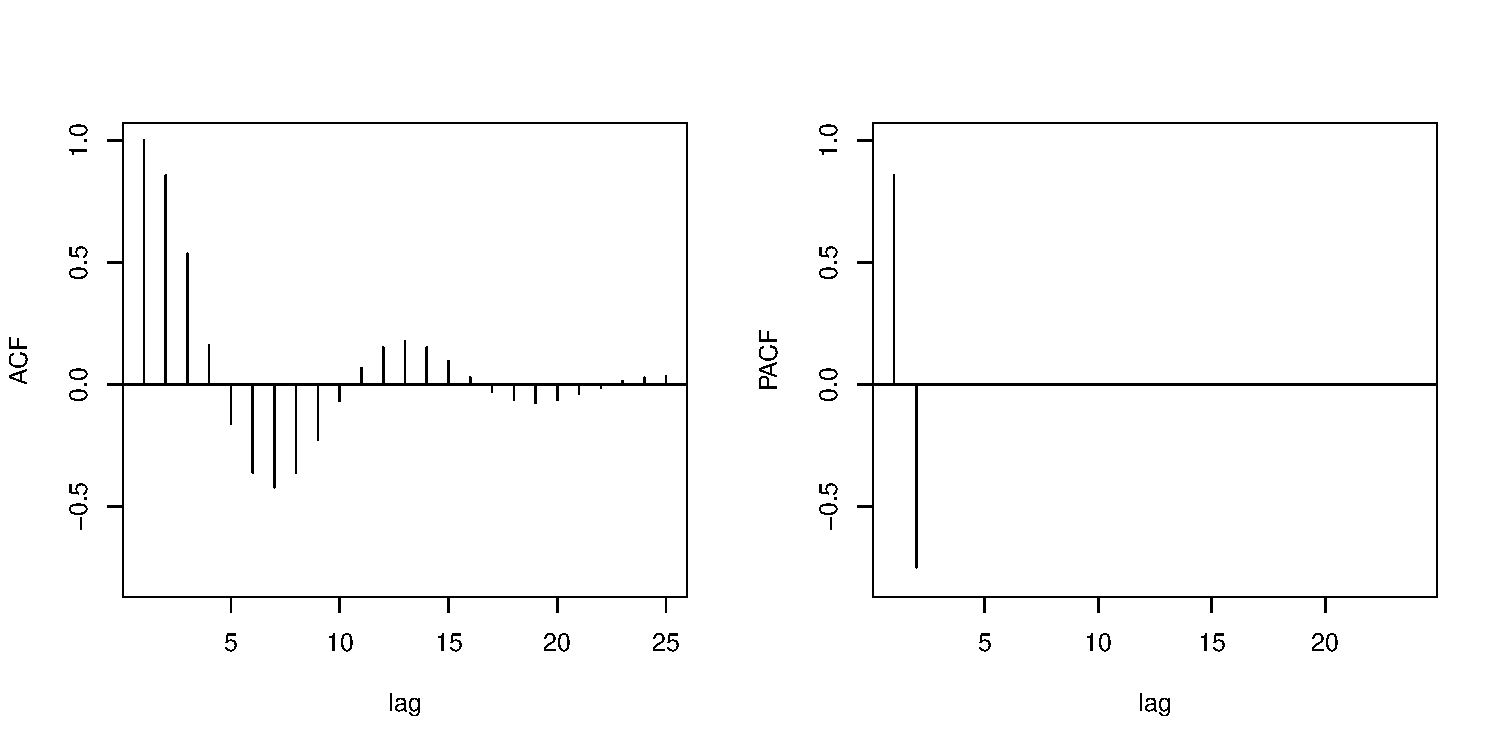
\includegraphics[width=\textwidth]{figure20.pdf}
\end{center}
\end{frame}

\begin{frame}{ARMA(p, q) Models -- Model Selection}
\small
\renewcommand{\arraystretch}{1.5}
\begin{tabular}{r|c|c|c} \hline
 & AR(p) & MA(q) & ARMA (p, q) \\ \hline
 ACF & Tails off & Cuts off after laq $q$ & Tails off \\
 PACF & Cuts off after lag $p$ & Tails off & Tails off \\ \hline
\end{tabular} \\

\vspace{\baselineskip}
\scriptsize Source: Shumway \& Stoffer, Table 3.1 \normalsize
\end{frame}


\begin{frame}{ARIMA(p, d, q) Models}

If the AR operator can be factorized by $(1-B)$, then:

\begin{align*}
\phi (B) = \left(1 - \sum_{j=1}^{p'} \phi_j B^j \right) = \left(1 - \sum_{j=1}^{p'-d} \phi_j B^j \right) (1 - B)^d 
\end{align*}

With $p=p'-d$, the \textbf{ARIMA(p,d,q)} model is then:

\begin{align*}
\left( 1 - \sum_{j=1}^p \phi_j B^j \right) (1-B)^d x_t &= \left( 1 + \sum_{j=1}^q \theta_j B^j \right) w_t
\end{align*}
%This can be generalized to:
%\begin{align*}
%\left( 1 - \sum_{j=1}^p \phi_j B^j \right) (1-B)^d x_t &= \delta + \left( 1 + \sum_{j=1}^q \theta_j B^j \right) w_t
%\end{align*} 
%where $\delta = \mu(1 - \phi_1 - \cdots - \phi_p)$

Here $(1-B)$ is the \textbf{differencing operator} $\nabla$. For example:

\begin{align*}
(1-\operatorname{B})x_t &= x_t - x_{t-1}  = \nabla x_t \\
(1-\operatorname{B})^2 x_t &= (1-2 \operatorname{B} + \operatorname{B}^2)x_t = x_t - 2x_{t-1} + x_{t-2} = \nabla^2 x_t\\
\cdots
\end{align*}

\end{frame}



\begin{frame}{Building ARIMA Models}
\begin{enumerate}
  \item Plot the data
  \item Possibly transform the data
  \item Assess stationarity
  \item Possibly difference the data
  \item Identify the dependence orders (p, q) of the model
  \item Estimate parameters
  \item Model diagnostics
  \item Model selection
\end{enumerate}
\end{frame}

\begin{frame}{Identifying Dependence Order}
\small
\begin{block}{Differencing \emph{d}}
\begin{itemize}
   \item Slow decay in sample ACF $\hat\rho(h)$ indicates need for differencing
   \item Over-differencing can introduce dependence where non exists
   \item Difference once using \texttt{diff(x, differences = 1)}, then check ACF again
\end{itemize}
\end{block}

\begin{block}{Preliminary \emph{p} and \emph{q}}
\begin{itemize}
   \item Examine sample ACF and PACF of differenced data % $\nabla^d x_t$
\end{itemize}
\vspace{.5\baselineskip} 
\renewcommand{\arraystretch}{1.5}
\begin{tabular}{r|c|c|c} \hline
 & AR(p) & MA(q) & ARMA (p, q) \\ \hline
 ACF & Tails off & Cuts off after lag $q$ & Tails off \\
 PACF & Cuts off after lag $p$ & Tails off & Tails off \\ \hline
\end{tabular} \\
\vspace{.5\baselineskip}
\scriptsize Source: Shumway \& Stoffer, Table 3.1 \normalsize
\end{block}
\end{frame}

\begin{frame}[fragile]{Example}
Examine data and transform:
\begin{Rcode}
# Plot data
plot(gnp)
# Plot ACF
acf2(gnp, 50)
# Log transform, and first order differencing
gnpgr = diff(log(gnp))
# Plot transformed and differenced data
plot(gnpgr)
# Plot ACF of transformed and differenced data
acf2(gnpgr, 24)
\end{Rcode}
\end{frame}

\begin{frame}{Example \small [cont'd]}
\begin{columns}
\begin{column}{0.15\textwidth}
\small
Original ACF and PACF
\end{column}
\begin{column}{0.75\textwidth}
\includegraphics[width=\textwidth]{figure22.pdf}
\end{column}
\end{columns}

\begin{columns}
\begin{column}{0.15\textwidth}
\small
Transformed and differenced ACF and PACF
\end{column}
\begin{column}{0.75\textwidth}
\includegraphics[width=\textwidth]{figure23.pdf}
\end{column}
\end{columns}
\end{frame}

\begin{frame}[fragile]{Example \small [cont'd]}
Fit initial models
\begin{Rcode}
# Fit an AR(1) model
sarima(gnpgr, 1, 0, 0)

# Fit an MA(2) model
sarima(gnpgr, 0, 0, 2)
\end{Rcode}
%\begin{Rcode}
%# Fit an AR(1) model
%sarima(gnpgr, 1, 0, 0)
%# Fit an MA(2) model
%sarima(gnpgr, 0, 0, 2)
%# Models are roughly equivalent
%ARMAtoMA(ar=0.35, ma=0, 10)
%\end{Rcode}

The models show similar fit and all coefficients are significant.
\end{frame}

\begin{frame}{Example \small [cont'd]}
\centering
\includegraphics[height=2.75in]{figure24.pdf}
\includegraphics[height=2.75in]{figure25.pdf}
\end{frame}

\begin{frame}{Example \small [cont'd]}
\begin{block}{Diagnostics}
\begin{itemize}
   \item Standardized residuals are normal random ($\mu=0$, $sd=1$)
   \item Residuals are not autocorrelated
   \item Residual ACF are random normal with $\mu=0$ and $sd=1/\sqrt{n}$
   \item Ljung-Box statistic $Q$ of the error ACF $\hat\rho_e$ for different maximum lags $H$ is larger than the $1-\alpha$ quantile of the $\chi^2_{H-p-q}$ distribution (i.e. the test statistic is not statistically signifantly different from $0$)
   %\begin{align*}
   %Q = n(n+2) \sum_{h=1}^H \frac{\hat\rho_e^2(h)}{n-h}
   %\end{align*}
\end{itemize}
\end{block}
\end{frame}

\begin{frame}[fragile]{Mis-Fit Example}
\begin{Rcode}
sarima(log(varve), 0, 1, 1, no.constant=T)
sarima(log(varve), 1, 1, 1, no.constant=T)
\end{Rcode}
\begin{center}
\includegraphics[height=2.5in]{figure26.pdf}
\includegraphics[height=2.5in]{figure27.pdf}
\end{center}
\end{frame}

\begin{frame}[fragile]{Example \small [cont'd]}
\begin{block}{Model Selection}
For MLE estimated models, model choice is typically based on information criteria
\begin{itemize}
   \item Functions of the log-likelihood $L$
   \item Adjusted for model complexity (number of parameters) $k$
   \item Adjusted for sample size $n$
   \item Express \emph{relative} quality of fit: \textbf{Smaller is better}
\end{itemize}
\begin{align*}
\operatorname{AIC} &= -2 \log L + 2k  &\qquad \text{\footnotesize Akaike Information Criterion}\\
\operatorname{AICc} &= AIC + \frac{2k(k+1)}{n-k-1} &\qquad \text{\footnotesize Akaike Information Criterion, corrected}\\
\operatorname{BIC} &= -2 \log L + k \log n &\qquad \text{\footnotesize Bayesian Information Criterion}
\end{align*}
\end{block}
\end{frame}

\begin{frame}[fragile]{Example \small [cont'd]}
\begin{textcode}
> sarima(gnpgr, 1, 0, 0)

AIC = -6.44694  AICc = -6.446693  BIC = -6.400958 
\end{textcode}

\begin{textcode}
> sarima(gnpgr, 0, 0, 2)

AIC = -6.450133  AICc = -6.449637  BIC = -6.388823 
\end{textcode}
\end{frame}


\begin{frame}[fragile]{Example -- Forecasting}
\begin{Rcode}
forecasts <- sarima.for(gnpgr, n.ahead=10, p=1,d=0,q=0)
\end{Rcode}
\begin{center}
\includegraphics[width=.75\textwidth]{figure21.pdf}
\end{center}
\vspace{-\baselineskip}
\begin{block}{}
\centering \small
ARMA predictions quickly settle to the mean with a constant prediction error
\end{block}
\end{frame}


%\begin{frame}{Pure Seasonal ARMA Models}
%\begin{align*}
%\Phi_P(B^s)x_t &= \Theta_Q(B^s)w_t
%\end{align*}
%with seasonal autoregressive and moving average operators
%\begin{align*}
%\Phi_P(B^s) &= 1 - \Phi_1 B^s - \Phi_2 B^{2s} - \cdots - \Phi_P B^{Ps} \\
%\Theta_Q(B^s) &= 1 + \Theta_1 B^s - \Theta_2 B^{2s} - \cdots - \Theta_Q B^{Qs} \\
%\intertext{where $s$ is the seasonal period, e.g. 4 for quarterly data, 12 for monthly data, 52 for weekly data, etc.}
%\end{align*}
%\end{frame}


%\begin{frame}{Pure Seasonal ARMA Models -- ACF and PACF}

%\renewcommand{\arraystretch}{1.5}
%\begin{tabular}{r|>{\centering}m{2.5cm}>{\centering}m{2.5cm}m{2.5cm}} \hline
 %& AR$(P)_s$ & MA$(Q)_s$ & \begin{center}ARMA$(P, Q)_s$\end{center} \\ \hline
 %ACF & Tails off at lags $ks$ & Cuts off after lag $Qs$ & \begin{center}Tails off at lag $ks$\end{center} \\
 %PACF & Cuts off after lag $Ps$ & Tails off at lag $ks$ & \begin{center}Tails off at lag $ks$\end{center} \\ \hline
%\end{tabular} \\

%\begin{itemize}
 %\item ACF and PACF at nonseasonal lags $h \neq ks$ are zero
%\end{itemize}
%\scriptsize Source: Shumway\&Stoffer, Table 3.3 \normalsize
%\end{frame}



%\begin{frame}{Mixed Seasonal ARIMA Models SARIMA(p,d,q)x(P,D,Q)\textsubscript{s}}
%Combine seasonal and non-seasonal AR and MA operators into a multiplicative seasonal autoregressive moving average model SARIMA$(p,d,q) \times (P,D,Q)$:

%\begin{align*}
%\Phi_P(B^s)\phi(B) x_t \nabla_s^D \nabla^d x_t = \delta + \Theta_Q(B^S)\theta(B)w_t
%\end{align*}

%with ordinary and seasonal difference components given by

%\begin{align*}
%\nabla^d = (1-B)^d \quad \text{and} \quad \nabla_s^D = (1-B^s)^D
%\end{align*}
%\end{frame}

%\begin{frame}[fragile]{Example SARIMA(0,1,1)x(0,1,1)\textsubscript{12} Model}
%\begin{align*}
%\nabla_{12} \nabla x_t &= \Theta(B^{12}) \theta(B) w_t 
%\intertext{or}
%(1-B^{12}) (1-B) x_t &= (1 + \Theta B^{12}) (1 + \theta B) w_t \\
%(1 - B - B^{12} + B^{13}) x_t &= (1 + \theta B + \Theta B^{12} + \Theta \theta B^{13}) w_t
%\end{align*}
%or in difference form
%\begin{align*}
%x_t = x_{t-1} + x_{t-12} - x_{t-13} + w_t + \theta w_{t-1} + \Theta w_{t-12} + \Theta \theta w_{t-13}
%\end{align*}
%\end{frame}

%\begin{frame}[fragile]{Pure Seasonal AR(1) Example}
%\begin{align*}
%(1- \Phi B^{12}) x_t = w_t \qquad \text{or} \qquad x_t = \Phi x_{t-12} + w_t
%\end{align*}
%Simulate data:
%\begin{Rcode}
%# 12 (monthly, seasonal) phi values of 0.9
%phi = c(rep(0,11),.9)
%# Simulate an AR model 
%sAR = arima.sim(list(order=c(12,0,0), ar=phi), n=37)
%# Convert to a time series with seasonal frequency
%sAR = ts(sAR, frequency=12)
%# Plot the simulated data
%plot(sAR, main='seasonal AR(1)', xlab="year", type='c')
%# Plot the theoretical ACF and PACF
%ACF = ARMAacf(ar=phi, ma=0, 100)
%PACF = ARMAacf(ar=phi, ma=0, 100, pacf=TRUE)
%plot(ACF,type="h", xlab="LAG", ylim=c(-.1,1))
%plot(PACF, type="h", xlab="LAG", ylim=c(-.1,1))
%\end{Rcode}
%\end{frame}

%\begin{frame}[fragile]{Pure Seasonal AR(1) Example \small [cont'd]}
%\begin{center}
%\includegraphics[height=3in]{figure29.pdf}
%\end{center}
%\end{frame}

%layout(matrix(c(1,1,2, 1,1,3), ncol=2))
%par(mar=c(3,3,2,1), mgp=c(1.6,.6,0))
%plot(sAR, axes=FALSE, main='seasonal AR(1)', xlab="year", type='c')
%Months = c("J","F","M","A","M","J","J","A","S","O","N","D")
%points(sAR, pch=Months, cex=1.25, font=4, col=1:4)
%axis(1, 1:4); abline(v=1:4, lty=2, col=gray(.7))
%axis(2); box()
%ACF = ARMAacf(ar=phi, ma=0, 100)
%PACF = ARMAacf(ar=phi, ma=0, 100, pacf=TRUE)
%plot(ACF,type="h", xlab="LAG", ylim=c(-.1,1)); abline(h=0)
%plot(PACF, type="h", xlab="LAG", ylim=c(-.1,1)); abline(h=0)

%\begin{frame}[fragile]{Example SARIMA(0,1)x(1,0)\textsubscript{12} Model \small [cont'd]}
%\begin{align*}
%x_t = \Phi x_{t-12} + w_t + \theta w_{t-1}
%\end{align*}
%\begin{Rcode}
%phi = c(0, 0, 0, 0, 0, 0, 0, 0, 0, 0, 0, .8)
%# Theoretical ACF/PACF
%ACF = ARMAacf(ar=phi, ma=-.5, 50)
%PACF = ARMAacf(ar=phi, ma=-.5, 50, pacf=TRUE)
%# Plot it
%par(mfrow=c(1,2))
%plot(ACF, type="h", xlab="LAG", ylim=c(-.4,.8))
%plot(PACF, type="h", xlab="LAG", ylim=c(-.4,.8))
%\end{Rcode}
%\end{frame}

%\begin{frame}{Example SARIMA(0,1)x(1,0)\textsubscript{12} Model \small [cont'd]}
%\centering
%\includegraphics[width=\textwidth]{figure30.pdf}
%\end{frame}


%\begin{frame}[fragile]{Example SARIMA}
%Consider the Air Passengers \texttt{AirPassengers} data set of monthly totals of international airlines passengers from 1949 to 1960.
%\begin{Rcode}
%x = AirPassengers
%# Log-transform data
%lx = log(x); 
%# Differencing
%dlx = diff(lx)
%# Seasonal differencing
%ddlx = diff(dlx, lag=12)
%# Plot all time series
%tsplot(cbind(x, lx, dlx, ddlx), gg=T, col=2:5)
%\end{Rcode}
%\end{frame}

%\begin{frame}{Example SARIMA \small [cont'd]}
%\centering
%\includegraphics[height=3in]{figure31.pdf}
%\end{frame}

%\begin{frame}[fragile]{Example SARIMA \small [cont'd]}
%Sample ACF and PACF
%\begin{Rcode}
%acf2(ddlx,50, gg=T, col=2, lwd=2)
%\end{Rcode}

%\begin{center}
%\includegraphics[height=2.5in]{figure32.pdf}
%\end{center}
%\end{frame}

%\begin{frame}{Example SARIMA \small [cont'd]}
%\begin{block}{Seasonal Component}
%\begin{itemize}
   %\item ACF cuts off at lag 1s (s=12)
   %\item PACF tails off at lags 1s, 2s, 3s, 4s, 
   %\item $\Rightarrow$ SMA(1), $P=0$, $Q=1$ in seasons ($s=12$)
%\end{itemize}
%\end{block}

%\begin{block}{Non-Seasonal Component}
%\begin{itemize}
   %\item Both ACF and PACF tail off at lower lags
   %\item $\Rightarrow$ ARMA(1,1) within the seasons, $p=q=1$
%\end{itemize}
%\end{block}
%\end{frame}

%\begin{frame}[fragile]{Example SARIMA \small [cont'd]}
%Try to fit ARIMA(1,1,1)x(0,1,1)\textsubscript{12} on log-transformed data:

%\begin{Rcode}
%sarima(lx, 1,1,1, 0,1,1,12)
%\end{Rcode}

%\begin{itemize}
   %\item AR parameter is not significant, 
   %\item Drop one parameter from within seasons part
%\end{itemize}

%\begin{Rcode}
%sarima(lx, 0,1,1, 0,1,1,12)
%sarima(lx, 1,1,0, 0,1,1,12)
%\end{Rcode}

%\begin{itemize}
   %\item Information criteria are better for ARIMA(0,1,1)x(0,1,1)\textsubscript{12} model
%\end{itemize}
%\end{frame}

%\begin{frame}{Example SARIMA \small [cont'd]}
%\centering
%\includegraphics[height=3in]{figure33.pdf}
%\end{frame}

%\begin{frame}[fragile]{Example SARIMA \small [cont'd]}
%Forecast data for twelve months:
%\begin{Rcode}
%sarima.for(lx, 12, 0,1,1, 0,1,1,12)
%\end{Rcode}
%\begin{center}
%\includegraphics[width=\textwidth]{figure34.pdf}
%\end{center}
%\end{frame}

\begin{frame}{General Autoregressive Conditional Heteroscedastic (GARCH) Models}
ARCH models the variance of a series of returns:
\begin{align*}
r_t = \frac{x_t - x_{t-1}}{x_{t-1}} \qquad \text{(''Return'')}
\end{align*}

\textbf{Example}: ARCH(1) Model -- The variance depends on the prior return.
\begin{align*}
r_t &= \sigma_t \epsilon_t \\
\sigma_t^2 &= \alpha_0 + \alpha_1 r_{t-1}^2
\end{align*}
where $\epsilon_t$ is Gaussian. 
%Rewrite as AR(1) model in $r_t^2$
%\begin{align*}
%r_t^2 = \alpha_0 + \alpha_1 r_{t-1}^2 + \eta_t
%\end{align*}
%where $\eta_t = \sigma_t^2(\epsilon_t^2-1)$.
\end{frame}

\begin{frame}[fragile]{Example: Combined AR(1) and ARCH(1) Model}
AR(1) Model with ARCH(1) Errors:
\begin{align*}
x_t = \phi_0 + \phi_1 x_{t-1} + \sigma_t \epsilon_t \quad \text{where} \quad \sigma_t = \alpha_0 + \alpha_1 x_{t-1}^2
\end{align*} 
Example: US GNP Data
\begin{Rcode}
u = sarima(diff(log(gnp)), 1, 0, 0)
acf2(resid(u$fit)^2, 20)
\end{Rcode}
Squared residuals may have some dependence.
\begin{Rcode}
library(fGarch)
summary(garchFit(~arma(1,0)+garch(1,0), diff(log(gnp))))
\end{Rcode}
\end{frame}

\begin{frame}{Example: Combined AR(1) and ARCH(1) Model}
\centering
\includegraphics[width=\textwidth]{figure35.pdf}
\end{frame}

\begin{frame}{ARCH Extensions}
\begin{block}{ARCH(q) Model}
Extend the ARCH(1) Model to multiple previous returns:
\begin{align*}
\sigma_t^2 = \alpha_0 + \alpha_1 r_{t-1}^2 + \cdots + \alpha_p r_{t-p}^2 = \alpha_0 + \sum_{i=1}^q \alpha_i r_{t-i}^2
\end{align*}
\end{block}

\begin{block}{GARCH(p, q) Model}
Variance depends also on prior variances:
\begin{align*}
\sigma_t^2 &= \omega + \alpha_1 r_{t-1}^2 + \cdots + \alpha_q r_{t-q}^2 \\
           & \qquad \qquad + \beta_1 \sigma_{t-1}^2 + \cdots + \beta_p \sigma_{t-p}^2 \\
           &= \omega + \sum_{j=1}^q \alpha_j r_{t-j}^2 + \sum_{j=1}^p \beta_j \sigma_{t-j}^2
\end{align*}
\end{block}
\end{frame}

\begin{frame}[fragile]{GARCH Example -- DJIA Returns}
\begin{Rcode}
library(fGarch)
# Log transform
djiar = diff(log(djia$Close))[-1]
# Fit an AR(1) + GARCH(1,1) model
djia.g <- garchFit(~arma(1,0)+garch(1,1), data=djiar)
# Show summary information
summary(djia.g)
# Different plots available
plot(djia.g, which=3)
\end{Rcode}
\end{frame}

\begin{frame}{ARCH Example -- DJIA Returns \small [cont'd]}{ACF}
\centering
\includegraphics[height=1.5in]{figure36.pdf}
\includegraphics[height=1.5in]{figure37.pdf}
\end{frame}

\begin{frame}[fragile]{GARCH Example -- DJIA Returns \small [cont'd]}{Results}
\begin{textcode}
         Estimate  Std. Error  t value Pr(>|t|)    
mu      8.585e-04   1.470e-04    5.842 5.16e-09 ***
ar1    -5.532e-02   2.023e-02   -2.735 0.006238 ** 
omega   1.610e-06   4.459e-07    3.611 0.000305 ***
alpha1  1.244e-01   1.660e-02    7.496 6.55e-14 ***
beta1   8.700e-01   1.526e-02   57.022  < 2e-16 ***
shape   5.979e+00   7.917e-01    7.551 4.31e-14 ***
---
Log Likelihood:
 8249.619    normalized:  3.27756 
\end{textcode}

\vspace{-\baselineskip}
\begin{center}
\includegraphics[height=1.75in]{figure38.pdf}
\end{center}
\end{frame}


%\begin{block}{Temporal Symmetry}
%Predictions forward in time is the same as prediction backward in time for stationary models.
%\end{block}
%\end{frame}


\begin{frame}{Appendix -- Basic Time Series Functions in R}
\footnotesize
\renewcommand{\arraystretch}{1.25}
\begin{tabularx}{\textwidth}{l|X} \hline
\texttt{filter} & Filters time series, through moving averages or autoregression \\
\texttt{lag} & Creates a lagged version of a time series by shifting the timebase back \\
\texttt{diff} & Creates lagged differences \\ 
\texttt{plot.ts} & Plot a time series \\
\texttt{ts.plot} & Plot multiple time series \\
\texttt{lag.plot} & Scatterplot of lagged values \\
\texttt{acf} & ACF and plot \\
\texttt{ccf} & CCF and plot \\ \hline
\end{tabularx}
\end{frame}

\begin{frame}{Appendix -- Basic Time Series Functions in R}
\footnotesize
\renewcommand{\arraystretch}{1.25}
\begin{tabularx}{\textwidth}{l|X} \hline
\texttt{time} & Creates the vector or times at which a time series was sampled \\
\texttt{cycle} & Gives the positions in the cycle of each observation \\
\texttt{frequency} & Number of samples per unit time \\
\texttt{ts.intersect} & Bind time series together that have a common frequency. Restrict to time covered by all series \\
\texttt{ts.union} & Bind time series together that have a common frequency. Pad with NA if necessary \\ 
\texttt{ar} & Fit an autoregressive model \\ 
\texttt{arima} & Fit an ARIMA model \\ \hline
\end{tabularx}
\end{frame}

\begin{frame}{Appendix -- Time Series Functions in the \texttt{astsa} library}
\footnotesize
\renewcommand{\arraystretch}{1.5}
\begin{tabularx}{\textwidth}{l|X} \hline
\texttt{tsplot} & Plot a time series \\
\texttt{acf1} & ACF and plot \\
\texttt{ccf2} & CCF and plot \\
\texttt{sarima} & Fit seasonal ARIMA models (and nice diagnostic plots) \\
\texttt{lag1.plot} & Scatterplot of lagged values \\ \hline
\end{tabularx}
\end{frame}



\end{document}



